\chapter{Recunoașterea obiectelor}


%Recunoașterea obiectelor este o aplicate fundamentala a procesării de imagini și viziunea artificiala.
%De câteva decenii a fost, și încă este un domeniu de cercetare extensiva.
%Termenul "recunoașterea obiectelor" este folosit pentru a descrie multe aplicații și algoritmi.
%Sensul comun, de cele mai multe ori, este: date fiind cunoștințe despre înfățișarea unor obiecte, una sau mai multe imagini sunt analizate pentru a se stabili dacă exista obiectele în imagine și locația lor.
%Cu toate acestea, fiecare aplicație are cerințe și constrângeri specifice.
%Acest fapt a condus la o mare diversitate de algoritmi.
%De aceea este important ca sa avem la îndemâna biblioteci software, care sa faciliteze dezvoltarea rapida a algoritmilor de recunoaștere a obiectelor.

%Un caz special de recunoaștere a obiectelor apare foarte des, baza de date a modelelor ce trebuiesc recunoscute conține o singura clasa de obiecte, în acest caz sarcina de a detecta prezenta obiectului în imagine este simplificata.

Problema recunoașterii de obiecte se poate exprima în felul următor: Având un o baza de date cu unul sau mai multe modele de obiecte, sa se determine dacă exista obiectul în imagine și dacă exista sa se localizeze.

Unele dintre cele mai relevante lucrări din domeniu sunt: 
\begin{itemize}
	\item "Robust Real-time Object Detection" \cite{Viola01robustreal-time}
	\item "Histograms of Oriented Gradients for Human Detection" \cite{Dalal05histogramsof}
	\item "Object Detection with Discriminatively Trained Part Based Models" \cite{Felzenszwalb_objectdetection}
\end{itemize}

Dacă studiem mai atent algoritmii descriși în aceste lucrări se observa ca toate au o structura comuna și urmăresc o succesiune de operațiuni similare.
Aceste operațiuni sunt următoarele: parcurgerea imaginii în scara și spațiu, extragerea de trăsături, clasificare și post-procesarea rezultatelor.

În continuare se va discuta mai detaliat despre fiecare componenta, iar la sfârșit despre algoritmul de recunoaștere.

\pagebreak
\section{Parcurgerea imaginii în scara și spațiu}

%Obiectele trebuie recunoscute la orice poziție și scara într-o imagine.
Obiectele care trebuiesc recunoscute pot prezenta deviații de la modelul din baza de date, aceste deviații pot fii de natura geometrica: translație, rotație, scalare și perspectiva.

O soluție pentru aceasta problema ar fii sa se construiască un model care sa prezinte toate instanțierile obiectului.
O dificultate cu aceasta abordare ar fii ca nu se pot știi dinainte toate transformările obiectului, chiar dacă s-ar știi, se poate deduce ca un astfel de model ar putea fii mult prea mare ca sa poată fii aplicat practic.

O alta abordare a fii sa se folosească o reprezentare a imaginii invarianta la aceste transformări.
Din literatura se știe ca o imagine reprezentata în spațiul Fourier este invarianta la translație și o imagine reprezentata în spațiul Log-Polar este invarianta la scalare și rotație.
Exista chiar și o combinație intre aceste doua reprezentări numita Fourier-Mellin care este invarianta la toate cele trei transformări.
Totuși s-a observat ca utilizarea acestei reprezentări are aplicații limitate, ea fiind folosita mai mult la alinierea imaginilor.

O alta soluție, poate un pic mai naiva, dar în același timp foarte puternica este folosirea unei combinații de piramida de imagini și un algoritm de tip fereastră glisantă\footnote{eng. sliding window}, acestea fiind aplicate pe imagine, nu pe modelul din baza de date.

Folosirea piramidei de imagini și fereastra glisanta ne permite ca in restul algoritmului de recunoaștere sa tratam problema ca și cum nu ar exista translații sau scalari, astfel simplificând mult algoritmii aplicați.

O piramida de imagini este o reprezentare multi-scara.
Piramida de imagini se formează, pornind de la o imagine sursa, prin scalari succesive.
Aceste scalari se fac cu un factor și se opresc atunci când se ajunge la o dimensiune minima.
Dacă factorul de scalare este ${\alpha > 1}$ atunci avem funcția care calculează dimensiunea unui nivel este  
$${ f(D,L) = D * \frac{1}{\alpha^L} }$$, unde ${D}$ este dimensiune imaginii sursa și ${L}$ este nivelul piramidei pentru care dorim sa aflam dimensiune.

Se poate vizualiza piramida de imagini în figurile următoare:

\begin{figure}[H]
	\centering
		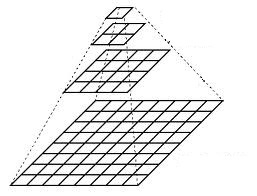
\includegraphics[width=0.90\textwidth]{imagini/Pyramids_Tutorial_Pyramid_Theory.png}
	\caption{Piramida de imagini}
	\label{fig:Pyramids_Tutorial_Pyramid_Theory}
\end{figure}

\begin{figure}[H]
	\centering
		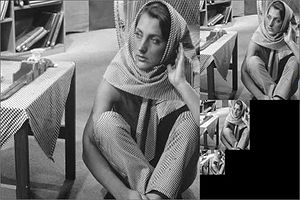
\includegraphics[width=0.90\textwidth]{imagini/300px-Example_pyramid.jpg}
	\caption{Exemplu piramida de imagini}
	\label{fig:300px-Example_pyramid}
\end{figure}


Prezentarea formarii piramidei de imagini în pseudo-cod:
\begin{mdframed}
\begin{verbatim}
sursa = citeste_imagine()
alpha = 6/5
dim_min = (100,100)
piramida = [sursa, ]
L=1
cicleaza
  D = sursa.D * 1/(alpha^L)
  daca D < dim_min
    atunci paraseste ciclul
  sfarsit daca
  nivel = scaleaza(sursa, D)
  piramida = insereaza(piramida, nivel)
  L = L + 1
sfarsit cicleaza
\end{verbatim}
\end{mdframed}

Se poate observa ca totuși acest model nu poate reprezenta toate scările posibile, fiind un model discret, aceasta problema poate fii ameliorata prin alegerea unui ${\alpha}$ potrivi și permițând modelului din baza de date sa reprezinte și el mici variații de scara.

O alta observație ar fii, cu cat ${\alpha}$ este mai mic, cu atât șansele sa nimerim scara corecta cresc, dar în același timp creste și consumul de memorie și durata de execuție a algoritmului. Consumul de memorie poate fii evitat dacă algoritmul se executa într-un mod recursiv, astfel eliminând menținerea explicita a unei liste de imagini în memorie.

Algoritmul fereastra glisanta se folosește pentru a obține invarianta la translație a modelului.
Aici fereastra se refera la o secțiune rectangulara a imaginii.
Fereastra va avea aceiași dimensiune ca și modelul din baza de date.
Fereastra glisanta are ca parametri ${\Delta_x, \Delta_y \geq 1}$, însemnând pasul pe axa x, respectiv pasul pe axa y.

Pseudo-cod fereastra glisanta:
\begin{mdframed}
\begin{verbatim}
dx = 8
dy = 8
I = citeste_imagine()
M = citeste_model()
pentru x de la 0 la latime(I) - latime(I)
  pentru y de la 0 la lungime(I) - lungime(M)
    fereastra = sectiune(I, x, y, latime(M), lungime(M))
    proceseaza(fereastra)
  sfarsit pentru
sfarsit pentru
\end{verbatim}
\end{mdframed}

Se observa ca și aici, ca și în cazul piramidei de imagini, cu cat x și y sunt mai mici cu atât creste și numărul de ferestre evaluate, ceea ce duce la un timp de execuție mai ridicat.

\pagebreak
\section{Extragerea de trăsături}

\pagebreak
\section{Clasificare}

\pagebreak
\section{Post-procesarea rezultatelor}

\pagebreak
\section{Algoritmul de recunoaștere}